
\documentclass[journal,12pt,twocolumn]{IEEEtran}
%

\usepackage{setspace}
\usepackage{gensymb}
\singlespacing
\usepackage{hyperref}
\usepackage{amsmath}
\usepackage{amsthm}
\usepackage{txfonts}
\usepackage{cite}
\usepackage{enumitem}
\usepackage{mathtools}
\usepackage{listings}
    \usepackage{color}                                            %%
    \usepackage{array}                                            %%
    \usepackage{longtable}                                        %%
    \usepackage{calc}                                             %%
    \usepackage{multirow}                                         %%
    \usepackage{hhline}                                           %%
    \usepackage{ifthen}                                           %%
  %optionally (for landscape tables embedded in another document): %%
    \usepackage{lscape}     
\usepackage{multicol}
\usepackage{chngcntr}
\renewcommand\thesection{\arabic{section}}
\renewcommand\thesubsection{\thesection.\arabic{subsection}}
\renewcommand\thesubsubsection{\thesubsection.\arabic{subsubsection}}

% correct bad hyphenation here
\hyphenation{op-tical net-works semi-conduc-tor}
\def\inputGnumericTable{}                                 %%

\lstset{
%language=C,
frame=single, 
breaklines=true,
columns=fullflexible
}

\begin{document}
%


\newtheorem{theorem}{Theorem}[section]
\newtheorem{problem}{Problem}
\newtheorem{proposition}{Proposition}[section]
\newtheorem{lemma}{Lemma}[section]
\newtheorem{corollary}[theorem]{Corollary}
\newtheorem{example}{Example}[section]
\newtheorem{definition}[problem]{Definition}
\newcommand{\BEQA}{\begin{eqnarray}}
\newcommand{\EEQA}{\end{eqnarray}}
\newcommand{\define}{\stackrel{\triangle}{=}}
\bibliographystyle{IEEEtran}
\providecommand{\mbf}{\mathbf}
\providecommand{\pr}[1]{\ensuremath{\Pr\left(#1\right)}}
\providecommand{\qfunc}[1]{\ensuremath{Q\left(#1\right)}}
\providecommand{\sbrak}[1]{\ensuremath{{}\left[#1\right]}}
\providecommand{\lsbrak}[1]{\ensuremath{{}\left[#1\right.}}
\providecommand{\rsbrak}[1]{\ensuremath{{}\left.#1\right]}}
\providecommand{\brak}[1]{\ensuremath{\left(#1\right)}}
\providecommand{\lbrak}[1]{\ensuremath{\left(#1\right.}}
\providecommand{\rbrak}[1]{\ensuremath{\left.#1\right)}}
\providecommand{\cbrak}[1]{\ensuremath{\left\{#1\right\}}}
\providecommand{\lcbrak}[1]{\ensuremath{\left\{#1\right.}}
\providecommand{\rcbrak}[1]{\ensuremath{\left.#1\right\}}}
\theoremstyle{remark}
\newtheorem{rem}{Remark}
\newcommand{\sgn}{\mathop{\mathrm{sgn}}}
\providecommand{\abs}[1]{\lvert#1\rvert}
\providecommand{\res}[1]{\Res\displaylimits_{#1}} 
\providecommand{\norm}[1]{\lVert#1\rVert}
\providecommand{\mtx}[1]{\mathbf{#1}}
% \providecommand{\mean}[1]{E\left[ #1 \right]}
\providecommand{\fourier}{\overset{\mathcal{F}}{ \rightleftharpoons}}
\providecommand{\system}{\overset{\mathcal{H}}{ \longleftrightarrow}}
\newcommand{\solution}{\noindent \textbf{Solution: }}
\newcommand{\cosec}{\,\text{cosec}\,}
\providecommand{\dec}[2]{\ensuremath{\overset{#1}{\underset{#2}{\gtrless}}}}
\newcommand{\myvec}[1]{\ensuremath{\begin{pmatrix}#1\end{pmatrix}}}
\newcommand{\cmyvec}[1]{\ensuremath{\begin{pmatrix*}[c]#1\end{pmatrix*}}}
\newcommand{\mydet}[1]{\ensuremath{\begin{vmatrix}#1\end{vmatrix}}}
\newcommand{\proj}[2]{\textbf{proj}_{\vec{#1}}\vec{#2}}
\newcommand{\RNum}[1]{\uppercase\expandafter{\romannumeral #1\relax}}
\let\StandardTheFigure\thefigure
\let\vec\mathbf
\title{
\LARGE SM5083\\
    \LARGE Assignment Number 01 \\[0.5em]
    
    \large Akash S. Kamble\par
    \large   SM21MTECH11002  \par
}
\maketitle
\renewcommand{\thefigure}{\theenumi}
\renewcommand{\thetable}{\theenumi}
\section{ Chapter \RNum{2}  Ex-14 Q. \RNum{2}}
\renewcommand{\theequation}{\theenumi}
\begin{enumerate}[label=\thesection.\arabic*.,ref=\thesection.\theenumi]
\numberwithin{equation}{enumi}
\item Problem Statement:Find the in-centres of the triangles whose vertices are as follows,
(5,3), (5,-1), (-7,-6)\\

\solution
let \begin{align}
    \vec{A} = \myvec{5\\3}, \vec{B} = \myvec{5\\-1},\vec{C}=\myvec{-7\\-6}\\
    B-A=\myvec{0\\-4}
\end{align}

\begin{align}
\norm{\vec{B}-\vec{A}}^2= (\vec{B}-\vec{A})^\top (\vec{B}-\vec{A})\;
&=  \myvec{0 \ -4} \myvec{0\\-4}\\
\norm{\vec{B}-\vec{A}}&=\sqrt{(0^2 + (-4)^2)}\\\nonumber
\norm{\vec{B}-\vec{A}}&=4\\
\end{align}
similarly,\\
\begin{align}
\norm{\vec{C}-\vec{B}}&=13\\
\norm{\vec{A}-\vec{C}}&=15
\end{align}
Now find in-centre of a triangle,\\
\begin{align*}
In-centre&=(\frac{\norm{\vec{B}-\vec{A}}C+\norm{\vec{C}-\vec{B}}A+\norm{\vec{A}-\vec{C}}B}{\norm{\vec{B}-\vec{A}}+\norm{\vec{C}-\vec{B}}+\norm{\vec{A}-\vec{C}}})\\
\\
&=(3.5,0)
\end{align*}


\begin{figure}[!ht]
	\centering
	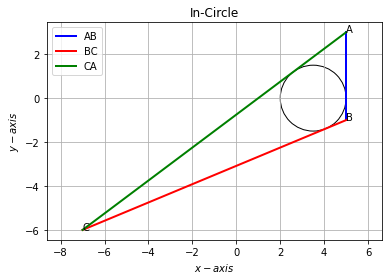
\includegraphics[width=\columnwidth]{incircle.png}
	\caption{A Triangle for given points}

\end{figure}

\end{enumerate}
\end{document}
